\chapter[Introduction]{Aimantation nucléaire}
\label{chap:intro}

\section{Généralités}
La résonance magnétique nucléaire a initialement été une méthode physique
d'investigation des propriétés magnétiques présentées par certains noyaux atomiques.
Les chimistes ont rapidement été convaincus de l'importance de cette technique 
lorsqu'a été établie la relation entre les fréquences de résonance des noyaux 
et la nature de leur environnement électronique, ouvrant
ainsi la voie vers une nouvelle méthode spectroscopique d'analyse.
Des progrès technologiques substantiels autorisent actuellement l'enregistrements de
spectres de molécules de haut poids moléculaire tels que les polymères d'origine
biologique.
Les techniques expérimentales de la RMN ont considérablement évolué au cours
du temps, à la fois vers la recherche de la meilleure sensibilité possible
et vers une assistance à l'interprétation.
La mesure de ces progrès peut être prise si on considère, par exemple, 
qu'il y a quelques décennies les chimistes des substances naturelles vérifiaient 
à l'aide d'un spectre de RMN à basse résolution les structures obtenues à l'issue de
complexes cascades de transformations chimiques.
Actuellement des structures de molécules organiques sont complètement déduites de
plusieurs types de spectres à haute résolution, 
à une ou deux (voire trois ou quatre) dimensions.

La RMN, au cours de son évolution, a conquis une grande variété d'utilisateurs.
Les chimistes des matériaux, et en particulier ceux des polymères, ont bénéficié de
la mise au point de techniques d'enregistrement adaptées aux échantillons solides qui
autorisent l'enregistrement de spectres à haute résolution.
L'interprétation des spectres de RMN des solides a aussi bénéficié de l'apport des
techniques bidimensionnelles.
L'étude par RMN des polymères biologiques à l'état solide est en plein essor méthodologique.

Le grand public ne connaît l'existence de la RMN que par les extraordinaires
images de l'intérieur du corps humain fournies par l'imagerie de résonance magnétique (IRM).
La RMN donne accès à
la concentration et la nature de l'environnement des molécules d'eau et des graisses
contenues dans les tissus biologiques.
La détection indirecte de la concentration de l'oxygène dans les 
tissus cérébraux a ouvert la voie
aux études d'imagerie fonctionnelle.
Des études métaboliques, par exemple en RMN du \phos, permettent de comprendre
et de diagnostiquer les dysfonctionnements musculaires.

Des applications particulières, telle la détermination de la teneur en eau d'un
matériau ou la mesure du comportement en fonction de la température d'une graisse,
sont de plus en plus souvent effectuées par RMN à basse résolution.
Ces méthodes d'analyse se développent particulièrement en milieu industriel.
La liste des applications possibles n'est certainement pas close à l'heure actuelle,
mais les principes sous-jacents sont établis dans leurs grandes lignes depuis l'époque
des premiers succès expérimentaux.

La suite de ce chapitre introductif présente un survol de notions élémentaires
nécessaires à la compréhension de la RMN impulsionnelle.
Ces notions seront approfondies au chapitre suivant, consacré lui aussi
à une description purement classique des phénomènes mis en jeu.

\section{Le magnétisme nucléaire}
Toutes les applications citées ci-dessus mettent en jeu les propriétés magnétiques
des noyaux atomiques.
La physique classique, celle de Newton et de Maxwell, est
incapable de rendre compte de ces propriétés.
L'exposé qui suit essaiera de rester intelligible aux non spécialistes de
la physique quantique en introduisant un minimum de concepts
étrangers au sens commun.

Un noyau atomique est constitué de protons et de neutrons, à l'exception du noyau de
l'atome d'hydrogène, constitué d'un unique proton.
Un noyau possède, comme toute particule, une masse et une charge électrique.
Il possède aussi un moment cinétique $\elvec$ 
et un moment magnétique $\aimvec$.
Ces deux grandeurs physiques caractérisent
un mouvement de rotation propre (sur elle-mêmes) des particules.
Une sphère homogène tournant sur elle-même possède un moment cinétique propre,
grandeur vectorielle dont les caractéristiques sont :
\begin{itemize}
\item sa norme, proportionnelle à la fréquence de rotation,
\item sa direction, identique à celle de l'axe de rotation,
\item son sens, défini de façon conventionnelle par le sens de déplacement d'un tire-
bouchon ordinaire qui serait solidaire de la sphère.
\end{itemize}
Rien en mécanique classique ne prédispose $\elvec$ à posséder des valeurs
particulières ni pour sa norme $\els$ ni pour la valeur algébrique $\elus$ de sa
projection sur un axe quelconque de vecteur directeur $\uvec$.
Le moment cinétique des noyaux atomiques, au contraire, possède une
norme qui ne dépend que de la nature du noyau considéré et $\elus$ ne peut
prendre qu'un nombre limité de valeurs.
La valeur de $\els$ se calcule à partir d'un
nombre entier ou demi-entier $I$ appelé nombre de spin (ou spin).
Les valeurs possibles de $\elus$ se déduisent du nombre $m_I$ vérifiant
\begin{equation}
-I \le m_I \le I
\end{equation}
où $m_I$ varie par valeurs entières. Ainsi :
\begin{eqnarray}
\els & = & \sqrt{I(I+1)}\hbar \\
\elus & = & m_I \hbar
\end{eqnarray}
La rotation interne des noyaux atomiques n'est pas mise en évidence de façon
directe mais elle est la cause de leur moment magnétique $\aimvec$,
grandeur vectorielle dont l'existence est révélée par l'interaction du noyau avec un
champ magnétique, comme indiqué ci-après.
Une spire de surface $S$ parcourue par un courant électrique d'intensité $i$ possède un
moment magnétique $\aimvec$,
représenté par un vecteur de norme $\aims$ égale au produit $iS$, de
direction normale à la surface de la spire et de
sens lié au sens de circulation du courant
électrique par la règle du tire-bouchon.

Un noyau atomique peut être assimilé à une sphère chargée.
Dans son mouvement de rotation interne,
chaque petit élément de volume de la sphère décrit une
trajectoire circulaire et peut donc être considéré comme équivalent
à une spire centrée sur l'axe de rotation,
perpendiculaire à cet axe et parcourue par un courant proportionnel
à la vitesse de rotation.
Cette image classique d'une sphère chargée en rotation est transposable,
avec les précautions d'usage, à l'échelle nucléaire.
Il en résulte l'existence pour un noyau atomique d'un moment magnétique,
mais possédant des propriétés particulières liées à la nature
même du moment cinétique sous-jacent.
Le moment magnétique est proportionnel au moment cinétique $\elvec$.
Le coefficient de proportionnalité est une
caractéristique du noyau appelée rapport gyromagnétique, notée $\gamma$.
Notons que cette grandeur peut être positive ou négative.
Cela indique bien qu'assimiler un noyau atomique à une sphère uniformément
chargée animée d'un mouvement classique de rotation n'est qu'une vue de l'esprit.
Par ailleurs, le neutron, de charge globale nulle, possède aussi un moment
magnétique.

$\aims$ et $\aimus$ (mesure algébrique de $\aimvec$
sur un axe quelconque dirigé par un vecteur $\uvec$de norme 1)
s'expriment en fonction de $I$ , $m_I$ et $\gamma$ :
\begin{eqnarray}
\aims & = & \gamma \sqrt{I(I+1)}\hbar \\
\aimus & = & \gamma m_I \hbar
\end{eqnarray}

Le moment magnétique d'une particule est mis en évidence par
son interaction avec un champ magnétique $\bzerovec$
d'intensité $\bzeros$.
Classiquement, un couple de forces de moment
$\Gammavec$ s'exerce sur la particule :
\begin{equation}
\Gammavec = \aimvec \wedge \bzerovec
\end{equation}
Ce couple s'annule lorsque $\bzerovec$ et $\aimvec$
ont même direction, ce qui se traduit par une absence
de variation du moment cinétique de la particule.
Elle est alors dans un état d'équilibre stable si
$\bzerovec$ et $\aimvec$ ont le même sens et
instable dans le cas contraire.
En effet, Le travail qu'il faut fournir pour faire passer le système
de moment magnétique $\aimvec$ d'un état de référence à un autre état définit l'énergie
d'interaction entre $\bzerovec$ et $\aimvec$.
L'état de référence choisi par convention est celui où $\bzerovec$ est nul.
L'expression classique de l'énergie d'interaction est alors
\begin{equation}
E = - \aimvec . \bzerovec
\end{equation}
qui est minimale lorsque $\bzerovec$ et $\aimvec$
ont mêmes sens et directions (équilibre stable) et maximale
lorsque $\bzerovec$ et $\aimvec$ sont de sens opposés
(équilibre instable).
L'expression de l'énergie d'interaction, établie d'après les lois de la physique
classique, reste valable pour les noyaux atomiques.
Ainsi,
\begin{equation}
E = - \aimzs.\bzeros
\end{equation}
si on désigne par $Oz$ l'axe ayant le sens et la
direction du champ magnétique et $\aimz$ la mesure algébrique
de la projection de $\aimvec$ sur cet axe.
E s'exprime en fonction de $m_I$
\begin{equation}
E = - m_I \gamma \hbar \bzeros
\end{equation}

La quantification de l'énergie d'un système, c'est-à-dire sa dépendance vis-à-vis d'un
paramètre variant de façon discontinue, est familière au chimiste, au moins en ce qui
concerne l'existence de niveaux énergétiques des électrons dans les atomes et les
molécules.
La figure \ref{fig:energie} illustre la répartition des niveaux énergétiques d'un
noyau de spin $I$ = 1.

\begin{figure}[hbt]
\begin{center}
\begin{pspicture}(0,-3)(5.5,2)
\SpecialCoor
\psline{->}(0.5,-2.5)(5.5,-2.5)
\uput[-90](5.5,-2.5){$B$}
\uput[-90](3.5,-2.5){$\bzero$}
\psline{->}(0,-2)(0,2)
\uput[180](0,2){$E$}
\uput[180](0,0){$0$}
\psline(0,0)(4.5,2)
\psline(0,0)(4,0)
\psline(0,0)(4.5,-2)
\psline[linewidth=0.1](!3 3.5 2 mul 4.5 div)(!4 3.5 2 mul 4.5 div)
\uput[0](!4 3.5 2 mul 4.5 div){$E_{-1}$}
\psline[linewidth=0.1](3,0)(4,0)
\uput[0](4,0){$E_{0}$}
\psline[linewidth=0.1](!3 3.5 2 mul 4.5 div neg)(!4 3.5 2 mul 4.5 div neg)
\uput[0](!4 3.5 2 mul 4.5 div neg){$E_{+1}$}
\psline[linestyle=dashed,linewidth=0.02,dash=3pt 3pt](3.5,2)(3.5,-2.5)
\end{pspicture}
\caption{\label{fig:energie}
\small Énergie d'une particule de spin 1 en interaction
avec un champ magnétique.}
\end{center}
\end{figure}

Parmi les noyaux de moment magnétique non nul, les noyaux de spin 1/2 jouent
un rôle particulier.
Dans cette catégorie figurent en effet les noyaux \prot, \carb, \azot,
\fluo et \phos présents principalement
dans les composés étudiés par les chimistes, biochimistes et biologistes.
De plus l'existence d'uniquement deux  niveaux énergétiques notés
$E_{\al}$ ($m_I = +1/2$) et $E_{\be}$ ($m_I = -1/2$) facilite
l'analyse des séquences impulsionnelles communément utilisées.

\section{La résonance}
Mettre en évidence expérimentalement les niveaux énergétiques d'interaction
entre un noyau et un champ magnétique revient à lui fournir l'énergie nécessaire pour
passer d'un état énergétique à un autre par l'intermédiaire d'une onde
électromagnétique (OEM).
Une OEM est constituée d'un champ électrique et d'un champ magnétique
variant de façon périodique, avec une fréquence notée $\nu$; elle ne peut échanger son
énergie avec la matière que par quantités finies $\Delta E$, appelées quanta
d'énergie, telles que
\begin{equation}
\Delta E = h \nu
\end{equation}
où $h$ est la constante de Planck ($6,63.10^{-34}$ J.s).
Cette condition n'est pas suffisante pour
réellement observer un saut (ou une transition) énergétique.
Il faut de plus que l'état initial et l'état final soient liés par les règles
de sélection.
Dans le cas qui nous intéresse il
faut que la transition énergétique s'accompagne d'une variation de $m_I$
telle que
\begin{equation}
\Delta m_I = \pm 1.
\end{equation}
Les seules transitions autorisées occasionnent une perte ou un gain d'énergie
\begin{equation}
\Delta E = \hbar \gamma \bzeros
\end{equation}
Pour observer ces
transitions il faut soumettre le noyau à une OEM de fréquence $\nu_0$ vérifiant
\begin{equation}
E = h \nu_0 = \hbar \omega_0 = \hbar \gamma \bzeros
\end{equation}
La quantité $\omega_0$ est la pulsation de l'OEM reliée à sa fréquence par
la relation
\begin{equation}
\omega_0 = 2 \pi \nu_0
\end{equation}
La condition de transition, appelée aussi condition de résonance s'écrit donc :
\begin{equation}
\label{equbase}
\omega_0 = \gamma \bzeros
\end{equation}
L'OEM agit sur le moment magnétique du noyau par le seul intermédiaire de son
champ magnétique variable noté $\bunvec$.
L'intensité maximale de ce champ est environ dix mille
fois plus faible que celle du champ statique $\bzerovec$.
Le fait qu'un champ si faible puisse faire passer le
noyau d'un état d'énergie particulier à un autre moins stable justifie le terme de
résonance, par analogie avec les résonances mécaniques ou électriques
où une excitation de faible amplitude appliquée à une fréquence convenable
est capable de provoquer des effets de grande amplitude.

Ce qui vient d'être écrit ne concerne qu'un noyau unique.
Il n'est pas question de détecter la résonance d'un seul noyau,
vue la faiblesse des énergies mises en jeu.
Pratiquement, la résonance est observée sur un échantillon macroscopique.
La notion de fréquence (ou de pulsation) de résonance,
introduite ici pour un noyau isolé reste correcte pour une
collection de noyaux identiques.

Pour que tous les noyaux identiques de l'échantillon aient la même fréquence de
résonance, c'est-à-dire pour que cette fréquence soit précisément mesurable, il faut
que l'intensité $\bzeros$ du champ soit la plus uniforme possible dans le
volume de l'échantillon.
En pratique, pour les applications de la RMN à haute résolution
$\Delta \bzeros/\bzeros$ est de l'ordre de $10^{-10}$.
Une telle homogénéité du champ est atteinte en corrigeant le champ magnétique
de l'aimant principal (permanent, électro--aimant résistif ou supraconducteur)
à l'aide d'électro--aimants supplémentaires désignés par le terme
anglais de "shims".
Pour un type de noyau donné la fréquence de résonance et l'intensité du champ
magnétique sont liés de façon univoque par la relation \ref{equbase}.
Par habitude, un spectromètre de RMN est traditionnellement
caractérisé par la fréquence de résonance du proton,
qui peut atteindre 1 GHz avec des aimants commerciaux.
Ces fréquences sont de l'ordre de grandeur de celles utilisées
pour les radio-transmission.
C'est pourquoi l'OEM excitatrice est aussi désignée sous le terme
de champ de radio-fréquences (RF).

\section{L'aimantation macroscopique}
\label{sec:macro}
La somme vectorielle des moments magnétiques individuels des différents
noyaux d'un échantillon macroscopique constitue le moment magnétique (ou
aimantation) total de cet échantillon.
La mise en résonance d'un noyau par une OEM
s'accompagne d'une variation du nombre $m_I$, dont dépendent à la fois
l'énergie d'interaction du noyau avec le champ magnétique $\bzerovec$
et la composante du moment magnétique sur l'axe $Oz$ du champ magnétique.
La mise en résonance de l'échantillon s'accompagne
donc d'une modification de son aimantation totale $\aimzerovec$.
Il est indispensable de comprendre comment $\aimzerovec$
varie sous différentes influences pour prévoir le résultat de
toute expérience de RMN.
Comme en mécanique, un système possédant un état initial
aussi bien caractérisé que possible évolue sous différentes contraintes.
Cette analogie a un grand intérêt puisque l'évolution du moment magnétique total d'un
ensemble de noyaux isolés (sans interaction magnétique mutuelle) est prévisible par
application des lois de la mécanique classique.
Seuls les ensembles de noyaux de spin $I = 1/2$ seront
traités à partir de ce point (sauf indication contraire).

$\aimzerovec$, pour un échantillon soumis
au seul champ $\bzerovec$ est un vecteur de même
direction que $\bzerovec$.
Dans cette situation les composantes de $\aimvec$
perpendiculaires à $\bzerovec$ pour
les différents noyaux sont réparties de façon aléatoire et s'annulent statistiquement.
Seule reste donc la somme des composantes des $\aimvec$
individuels parallèles à $\bzerovec$,
c'est-à-dire la somme $\aimzerovecz$ des projections individuelles.

L'échantillon est aussi en interaction avec l'extérieur par l'intermédiaire
d'échanges thermiques.
L'extérieur joue le rôle de thermostat de température absolue $T$.
Le nombre de noyaux (aussi appelé population) correspondant à chaque état
énergétique est alors gouverné par la loi de Boltzman :
la population $p$ d'un état d'énergie $E$ est proportionnelle à $\exp(-E/kT)$.
Dans le cas particulier des particules de spin 1/2,
on notera $p_{\al}$ et $p_{\be}$ les populations des états d'énergies
$E_{\al}$ et $E_{\be}$ associés au valeurs +1/2 et -1/2 de $m_I$.
\label{page:population}
Avec comme hypothèse que $\gamma$ est de signe positif,
$E_{\al}$ est inférieure à $E_{\be}$, et donc $p_{\al}$ est supérieur à $p_{\be}$.
\begin{eqnarray}
p_{\al} & = & K e^{-E_{\al}/kT} = K e^{+\gamma \hbar \bzeros/2kT} \\
p_{\be} & = & K e^{-E_{\be}/kT} = K e^{-\gamma \hbar \bzeros/2kT}
\end{eqnarray}
Le facteur de proportionnalité $K$ se déduit du nombre total $P$ de
noyaux de l'échantillon, sachant que
\begin{equation}
p_{\al} + p_{\be} = P
\end{equation}
A la température ambiante (300 K par exemple), et même aux valeurs les
plus élevées possibles de $\bzeros$ que l'on utilise pratiquement,
$\gamma \hbar \bzeros/2kT$ est de l'ordre de $10^{-5}$.

En approximant alors $\exp(x)$ par $1+x$,
\begin{eqnarray}
p_{\al} & = & P/2.(1+\gamma \hbar \bzeros/2kT) \\
p_{\be} & = & P/2.(1-\gamma \hbar \bzeros/2kT)
\end{eqnarray}
Le facteur $K$ vaut en effet $P/2$ pour que l'égalité
$p_{\al} + p_{\be} = P$ soit bien vérifiée.
Sachant que $p_{\al}$ (resp. $p_{\be}$) noyaux présentent une composante
$\aimz$ de leur moment magnétique sur l'axe $O_z$
égale à $1/2.\gamma \hbar$ (resp. $-1/2.\gamma \hbar$) :
\begin{equation}
\label{eqn:diffpopgamma}
\aimzerozs = 1/2. \gamma \hbar (p_{\al} - p_{\be}) =
P \gamma^2 \hbar^2 \bzeros / 4kT
\end{equation}
L'importance de la quantité $p_{\al} - p_{\be}$, appelée différence de population
$\Delta P$, se comprend aisément si on considère que l'intensité de
l'absorption d'une OEM par l'échantillon est d'autant plus grande
qu'il y a de noyaux à faire évoluer de l'état fondamental vers l'état
d'énergie plus élevé.

\ignore{
Ce point mérite d'être précisé avec un peu plus de finesse.
L'onde électromagnétique induit des transitions de l'état $m_s = +1/2$ vers l'état $m_s = -1/2$
avec une probabilité par unité de temps $\transpm$, et de l'état $m_s = -1/2$ 
vers l'état $m_s = +1/2$ avec une probabilité par unité de temps $\transmp$.
On peut montrer par ailleurs que $\transpm = \transmp$ et qui sera notée $W$.
Pour l'état $m_s = +1/2$, on peut donc écrire l'équation d'évolution :
\begin{equation}
\frac{\mbox{d}p_+}{\mbox{d}t} = -\transpm p_+ + \transmp p_- = -W (p_+ - p_-) = -W \cdot \Delta p
\end{equation}
et que parallèlement
\begin{equation}
\frac{\mbox{d}p_-}{\mbox{d}t} = +W \cdot \Delta p
\end{equation}
conduisant à 
\begin{equation}
\frac{\mbox{d} \Delta p}{\mbox{d}t} = -2W \cdot \Delta p
\end{equation}
La différence de population décroît donc de sa valeur initiale jusqu'à atteindre 0,
ce qui correspond à la situation d'égalité des populations, aussi appelée saturation.
A partir du moment où les populations sont égales, il devient impossible
de mettre en évidence la possibilité d'une transition énergétique.
L'absorption d'énergie par l'échantillon n'est perceptible que de manière transitoire
et pendant un temps d'autant plus court que $W$ est grand et donc que l'intensité de l'onde
électromagnétique est grande.
La situation est en fait plus complexe car la saturation ne correspond pas à un état
d'équilibre de l'échantillon, état vers lequel il est ramené 
par les phénomènes de relaxation (voir ci-après).
}

Le vecteur $\aimzerovec$ reste aligné avec l'axe $Oz$
tant que la seule action magnétique subie par l'échantillon est celle due
au champ $\bzerovec$.
On désignera par la suite par $\aimvec$ l'aimantation totale de l'échantillon
dans le cas général, sachant qu'il ne sera plus fait référence
aux moments magnétiques individuels des noyaux.
L'action supplémentaire exercée par l'OEM se
traduit par la création d'un état hors-équilibre où
$\aimvec$ et $\bzerovec$ font un angle $\theta$ non nul.
Lorsque l'aimantation totale  n'est plus celle de l'état d'équilibre,
son évolution est décrite par les équations de la mécanique classique en considérant
le mouvement d'une sphère de moment magnétique $\aimvec$, de
moment cinétique $\elvec$,
tel que $\aimvec = \gamma \elvec$,
plongée dans le champ $\bzerovec$.
Les lois de la mécanique classique, appliquées à cet objet macroscopique,
indiquent que $\aimvec$ tourne
autour de l'axe $Oz$ à la pulsation $\omega_0 = \gamma \bzero$,
précisément égale à la pulsation de l'OEM capable
d'induire des sauts énergétiques.
Ce mouvement de rotation est appelé précession de Larmor.

\ignore{
L'OEM est créée par une paire de spires d'axe perpendiculaire à l'axe $O_z$
(ce sera l'axe $O_x$ par convention) placée au voisinage immédiat de l'échantillon.
Après avoir supprimé l'émission de l'OEM, $\aimvec$ continue son
mouvement de précession et sa variation au cours du temps crée dans ces spires
une tension induite proportionnelle à la vitesse de variation de
$\aimx$, valeur algébrique de la projection de
$\aimvec$ sur l'axe $O_x$.
En considérant que $\aimx$ vaut au maximum $\aimzeroz$
(pour $\theta = \pi/2$) et en prenant pour origine des temps ($t = 0$)
l'instant où $\aimvec$ évolue librement à partir
d'une direction faisant un angle $\phi$ avec l'axe $Ox$
\begin{equation}
\aimx(t) = \aimzeroz \cos(\omega_0 t + \phi).
\end{equation}
En considérant que la précession est infiniment plus rapide que la relaxation,
la tension $e$ induite dans les spires :
\begin{equation}
e(t) \propto \aimzeroz \omega_0 \sin(\omega t + \phi)
\end{equation}
a une valeur maximale proportionnelle à $\omega$ et à $\aimzeroz$.
Si $\omega_0$ et $\aimzeroz$ sont exprimés en fonction
de $\gamma$ et $\bzero$, $e$ est proportionnelle à $P$, à $\gamma^3$ et à
$\bzero^2$.
La grandeur $e$ étant la grandeur physique effectivement mesurée,
il est clair que pour un noyau de rapport gyromagnétique donné,
la résonance sera d'autant plus facilement détectée que l'échantillon
contiendra un grand nombre de noyaux et que $\bzero$ sera intense.
}

L'OEM est crée par une paire de spires d'axe perpendiculaire à l'axe $Oz$
(ce sera l'axe $Ox$ par convention) placée au voisinage immédiat de l'échantillon.
Après avoir supprimé l'émission de l'OEM, $\aimvec$ continue son
mouvement de précession et sa variation au cours du temps crée dans ces spires
une tension induite proportionnelle à la vitesse de variation de
$\aimx$, valeur algébrique de la projection de
$\aimvec$ sur l'axe $Ox$.
En considérant que $\aimx$ vaut au maximum $\aimzerozs$
(pour $\theta = \pi/2$) et en prenant pour origine des temps ($t = 0$)
l'instant où $\aimvec$ évolue librement à partir
d'une direction faisant un angle $\phi$ avec l'axe $Ox$
\begin{equation}
\aimxs(t) = \aimzerozs \cos(\omega_0 t + \phi).
\end{equation}
La tension sinusoïdale $e(t)$ induite dans les spires 
a une valeur maximale proportionnelle à $\omega_0$ et à $\aimzerozs$.
Si $\omega_0$ et $\aimzerozs$ sont exprimés en fonction
de $\gamma$ et $\bzeros$, $e$ est proportionnelle à $P$, à $\gamma^3$ et à
$\bzeros^2$.
La grandeur $e$ étant la grandeur physique effectivement mesurée,
il est clair que pour un noyau de rapport gyromagnétique donné,
la résonance sera d'autant plus facilement détectée que l'échantillon
contiendra un grand nombre de noyaux et que $\bzeros$ sera intense.

Les spires qui entourent l'échantillon constituent la partie inductive
circuit oscillant qui contient par ailleurs un condensateur électrique.
Ce circuit constitue un résonateur qui amplifie par un facteur $Q$, appelé
facteur de qualité, la tension induite par la variation de $\aimx$.
L'amplification obtenue est de même nature que celle fournie
par la caisse de résonance d'un violon : le son qu'il produit
est bien plus intense que celui émis par une corde tendue en l'air.
La résonance magnétique est en fait détectée grâce à une résonance électrique.

Ce qui est présenté ci-dessus peut laisser penser que $\aimvec$ reste
indéfiniment dans un état hors équilibre après absorption de l'OEM.
Des processus appelés mécanismes de relaxation font que $\aimvec$
retournera à son état d'équilibre $\aimzerovec$ dans le champ $\bzerovec$.
En conséquence, les écarts des composantes transversales
(perpendiculaires à $\bzerovec$) et longitudinales
(parallèles à $\bzerovec$) de $\aimvec$ par
rapport à leurs valeurs d'origine diminuent selon une loi exponentielle.
Cette décroissance est gouvernée par deux paramètres appelés temps de relaxation
longitudinal (noté $T_1$) et transversal (noté $T_2$).
Le courant induit dans les spires par l'existence de la force électromotrice
induite peut, s'il est très intense, favoriser le retour de l'aimantation
vers l'équilibre.
Ce phénomène est désigné sous le terme de \emph{radiation damping}
et est produit par exemple si l'échantillon contient un solvant protonné.

La figure \ref{fig:retour} montre la trajectoire de l'aimantation
macroscopique depuis un état initial où elle se trouve
dans le plan perpendiculaire à $\bzerovec$
jusqu'à son retour à l'équilibre.

\begin{figure}[hbt]
\begin{center}
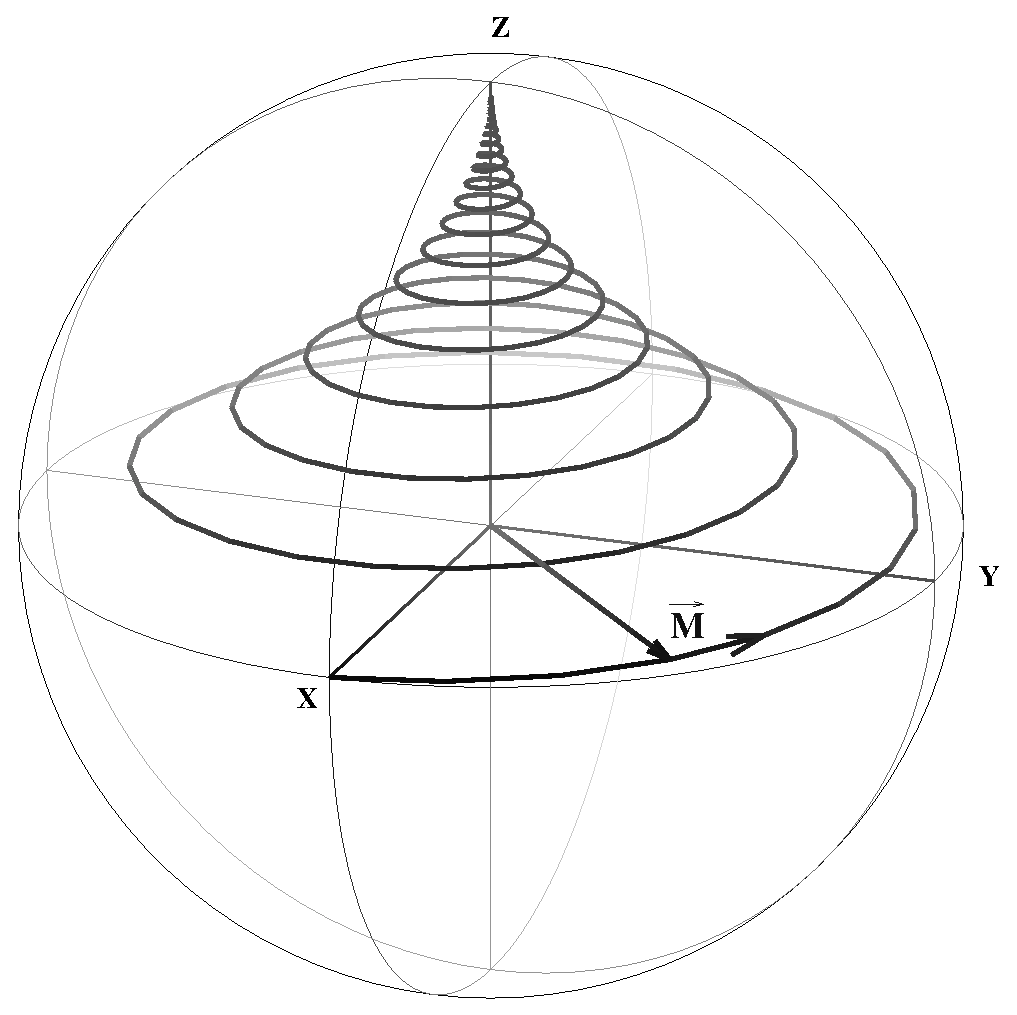
\epsfig{file=retour.eps,width=4in}
\end{center}
\caption{Retour à l'équilibre de l'aimantation macroscopique.}
\label{fig:retour}
\end{figure}

\section{Impulsions et onde continue}
Les noyaux de la même nature présents dans un échantillon n'ont généralement
pas tous la même fréquence de résonance, en particulier à cause de
l'effet différencié des électrons qui entourent les noyaux
(voir section \ref{sec:chemshift}).
Deux stratégies ont été successivement envisagées pour détecter et mesurer ces
différentes résonances et se traduisent par deux
façons différentes de manipuler le vecteur $\aimvec$ :
il s'agit des méthodes dites "par onde continue" et "par impulsion".
Cette dernière correspond à ce qui vient d'être présenté, à
savoir que $\aimvec$ est écarté de sa position initiale
et que $e(t)$ est analysée pendant la phase de retour à la situation initiale.
Sous réserve que la durée $T$ de la mise hors équilibre soit
suffisamment courte, et plus exactement que $1/T$ soit grand devant l'étendue de la
gamme de fréquences à considérer, tous les noyaux résonnant aux fréquences voisines
de celle de l'OEM subissent une perturbation identique.
La tension $e(t)$ recueillie aux bornes des spires au cours du retour
à la situation initiale est une somme de tensions
sinusoïdales de fréquences, d'amplitude et de phases différentes.
Le traitement de $e(t)$ nécessite des opérations de changement de fréquence
(toutes les fréquences sont diminuées d'une même quantité par un dispositif
électronique afin d'en faciliter le traitement ultérieur),
d'échantillonnage ($e(t)$ est mesurée à des intervalles de temps
réguliers) et de conversion analogique-digitale
(les résultats des mesures de $e(t)$ sont
converties en nombres binaires).
Il en résulte un ensemble de valeurs numériques,
manipulables par un calculateur,
qui contient toute l'information présente dans $e(t)$.
Pour un spectre de RMN du proton enregistré dans des conditions standard,
le temps nécessaire à l'acquisition des données est inférieur à 5 secondes.
L'analyse harmonique de $e(t)$ (sous forme numérique) est ensuite réalisée :
on obtient pour chaque fréquence l'intensité de la résonance.
Formellement, une fonction du temps $e(t)$ a été convertie en une fonction $S(\omega)$
appelée spectre.
Dans la pratique, le signal numérisé $S(\omega)$ se déduit de $e(t)$ par
transformation de Fourier, opération mathématique qui est calculée à l'aide
d'algorithmes rapides.

Pour des raisons technologiques, la recherche des
fréquences de résonance s'est d'abord effectuée
en faisant varier régulièrement et de façon
lente la fréquence $\nurf$ de l'OEM excitatrice.
L'absorption d'énergie est détectée par la mesure du
coefficient de surtension d'un circuit oscillant dont l'élément inductif est la bobine
d'excitation.
Une solution plus simple encore techniquement consiste à maintenir
constante la fréquence de l'OEM excitatrice et de faire varier régulièrement l'intensité
du champ magnétique $\bzeros$.
Pour obtenir un spectre de bonne qualité, il faut que $\bzeros$ ou $\nurf$ varie
lentement.
Typiquement, un spectre de proton standard était enregistré en 10 minutes
environ.

Le développement des techniques impulsionnelles se comprend aisément lorsque
l'on compare les possibilités d'amélioration du rapport signal/bruit des spectres.
Pendant les 10 minutes de l'enregistrement du spectre par la méthode de l'onde
continue, il est possible de répéter $N$ fois ($N = 100$, par exemple) le cycle
impulsion-acquisition et de co-additionner les valeurs de $e(t)$
(mises sous forme numérique) pour chaque valeur de $t$.
Une telle manipulation augmente dans un facteur $N$ le signal réellement
dû à la réponse des molécules et par un facteur $\sqrt{N}$ le bruit de fond crée par
les circuits électronique et dont la nature est aléatoire.
Le rapport Signal sur bruit (S/B) est amélioré dans un rapport $\sqrt{N}$
(soit 10 dans l'exemple choisi).
Il a été néanmoins possible d'améliorer aussi le rapport S/B
des spectre en onde continue en additionnant des spectres enregistrés successivement
dans les mêmes conditions.
L'obtention de spectres de \carb en abondance naturelle est
pratiquement irréalisable sans faire appel à l'accumulation rapide de spectres telle
qu'elle est effectuée par la méthode impulsionnelle.

L'élaboration d'expériences où les noyaux atomiques ne sont pas sollicités par
une seule impulsion mais par des trains (ou séquences) d'impulsions séparés par des
délais fixes ou variables, ouvre la voie à des méthodes d'investigation structurale
extrêmement puissantes.
Ces méthodes n'ont pas leur équivalent dans le domaine de
l'enregistrement en onde continue et s'appliquent aux molécules en solution, à l'état
solide et en imagerie médicale.

\section{Déplacement chimique, couplages}
\label{sec:chemshift}
Ce qui précède pourrait laisser penser que pour un type de noyau donné,
caractérisé par son rapport gyromagnétique la fréquence de résonance n'est déterminé
que par l'intensité $\bzeros$ du champ magnétique.
Si cela était réellement le cas la RMN serait restée une curiosité de
laboratoire, un peu comme si en spectroscopie infra-rouge toutes les fréquences de
vibration moléculaire correspondaient à un nombre d'onde de 3000 cm$^{-1}$.

Les électrons entourant un noyau créent un champ magnétique supplémentaire
sous l'influence du champ $\bzerovec$.
Il en résulte que le champ magnétique réellement perçu
par le noyau, $\bzerovecloc$, dépend de la densité électronique au
voisinage de ce noyau.
L'environnement chimique d'un noyau, c'est à dire la nature des atomes et des liaisons
environnantes est donc traduite par des valeurs particulières de
$\bzerolocs$.

$\bzerolocs$ est plus faible que $\bzeros$ et la différence est
proportionnelle à $\bzeros$.
Le facteur de proportionnalité est appelé constante d'écran (les électrons font écran
à $\bzerovec$ et noté $\sigma$ :
\begin{equation}
\bzerolocs = \bzeros(1-\sigma).
\end{equation}
La relation entre $\sigma$ et la fonction de densité électronique est connue
de manière théorique et les calculs correspondants sont réalisables en quelques minutes
pour des molécules peu complexes (quelques dizaines d'atomes) sur des ordinateurs
accessibles aux centres académiques.

Le coefficient $\sigma$ varie le plus souvent dans un intervalle restreint,
de 10$^{-5}$ pour les protons, de 2.10$^{-4}$ pour les noyaux de $^{13}$C.
La grandeur utilisée pratiquement n'est pas $\sigma$ mais le déplacement chimique
noté $\delta$, défini par rapport à la fréquence de
résonance d'un noyau d'une substance de référence comme le tétraméthylsilane
(TMS) pour les noyaux \prot et \carb.
La grandeur $\delta$ est sans unité :

\begin{equation}
\delta = \frac{\nu - \nutms}{\nutms}\times 10^6.
\end{equation}
L'usage a fait de $\delta$ une grandeur exprimée en ppm, ou parties par million.

L'existence d'un déplacement chimique bien défini présuppose que $\sigma$ ne dépend
pas de l'orientation relative de la molécule et de $\bzerovec$.
Ceci est faux en général, mais en phase liquide seule
une valeur moyenne de $\sigma$ est observée.
L'effet d'écran n'est décrit correctement qu'à
l'aide d'une matrice (ou tenseur) d'écran.

Le spectre de proton d'un composé organique en solution présente généralement
beaucoup plus de raies qu'il n'y a de type de protons chimiquement différents.
Cela est dû à une interaction magnétique entre noyaux appelée couplage scalaire
et dont le médiateur est le nuage électronique qui entoure les noyaux.
L'interaction magnétique directe à travers l'espace, appelée couplage
dipolaire, possède une moyenne nulle en milieu liquide isotrope mais est responsable
en partie des phénomènes de relaxation.
Dans les solides, le caractère tensoriel de l'effet d'écran et
le couplage dipolaire extrêmement intense (par comparaison
avec les couplages scalaires) donnent lieu à des spectres très complexes
qui peuvent être simplifiés par des techniques dédiées.

Les chapitres suivants seront essentiellement consacrés à la manipulation
de l'aimantation d'un échantillon sous l'influence de
$\bzerovec$, des couplages scalaires, ainsi que du
champ électromagnétique excitateur.
Ils constituent une base de connaissance nécessaire à la compréhension
des expériences usuelles utilisées pour l'analyse structurale
des molécules.

